\chapter{Prozess Architekturplanung}
Aufbauend auf den im Anforderungsprozess ermittelten Attribute, kann nun mit der Architekturplanung begonnen werden. Bereits an dieser Stelle können aufgrund der ermittelten Parameter und Erfahrungswerte eine grundsätzliche Überprüfung der Machbarkeit des Projektes durchgeführt werden. Auch eine Überprüfung, ob der beschriebene Prozess der Architekturplanung für das Projekt eignet kann durchgeführt werden: Der Prozess beschäftigt sich hauptsächlich mit der Aufspaltung und Trennung der Daten und Akteure in mehrere Systeme. Durch außergewöhnlich strenge Laufzeitanforderungen oder entsprechende Rahmenbedinungen kann diese Aufspaltung jedoch zu einer Architektur führen, welche die ursprünglich ermittelten Anforderungen nicht mehr, oder nur schlecht erfüllt.

\section{Erstellen der Minimalen Architektur}
Das Kontextdiagramm, welches im Anforderungsprozess erstellt worden ist, zeigt das System mit allen AkteurInnen und Nachbarsystemen. Aufbauend darauf kann nun die minimale Architektur erstellt werden, welche sich aus dem System und den Nachbarsystemen ableitet.

\begin{figure}[H]
    \centering
    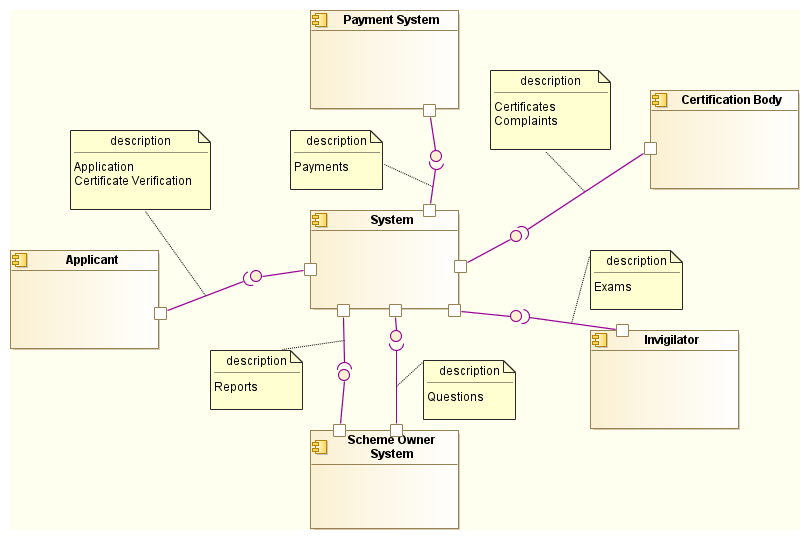
\includegraphics[scale=0.5]{uml/context.png}
    \caption{Das Kontextdiagramm liefert die Ausgangsbasis für die Architektur}
\end{figure}

Zuerst werden alle Datenflussnotizen entfernt. Danach werden alle Komponenten entfernt, welche kein eigenes System darstellen. In diesem Falle werden folgende Komponenten entfernt:

\begin{itemize}
  \item Applicant
  \item Certification Body
  \item Invigilator
\end{itemize}

Dies führt zu folgender Minimalarchitektur:

\begin{figure}[H]
    \centering
    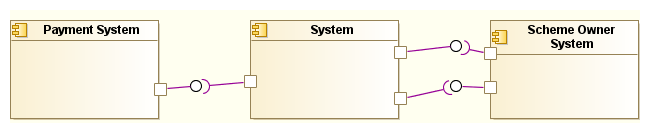
\includegraphics[scale=0.7]{uml/minimalarch.png}
    \caption{Minimale Architektur}
\end{figure}

Für die Nachbarsysteme selbst wird keine Architektur erstellt, jedoch beeinflussen sie die Schnittstellen des Systems und sind deswegen wichtig für den weiteren Prozess. Sie werden in die Architektur einbezogen.

\section{Erstellen der Datenminimalarchitektur}
Auf Basis der im Anforderungsprozess ermittelten Zonen wird das System der vorher erstellte Minimalarchitektur in ebenso viele Teilsysteme unterteilt. Die Aktivitätsdiagramme werden an die neue Architektur angepasst: Für jedes Untersystem wird in den Diagrammen eine eigene Swimlane erstellt. Die involvierten AkteurInnen sind, falls möglich, als eigene Swimlane modelliert, spielen in dieser Phase aber noch keine wichtige Rolle zur Gliederung des Systems.

\begin{figure}[H]
    \centering
    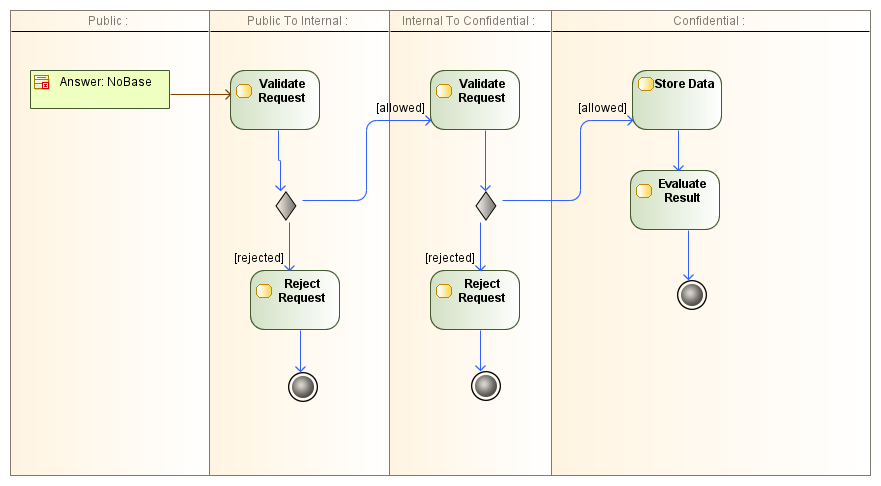
\includegraphics[scale=0.5]{uml/takeexamactivity1.png}
    \caption{Die Antworten werden nach der Prüfung an den Certification Body übermittelt. Der Request wird dann durch zwei Gateways zum finalen System geleitet.}
\end{figure}

Wechselt der Kontrollfluss eine Swimlane eines Systems, heißt dies, dass eine Verbindung zwischen den beiden sonst abgeschotteten Systemen benötigt wird. Dieses Verbindung wird als eigene Komponente modelliert und wird als Gateway bezeichnet. Die Aufgabe dieses Gateways ist es, folgende Attribute der Anfrage zu überprüfen und die Anfrage gegebenenfalls zu verwerfen oder weiterzuleiten:

\begin{itemize}
  \item Von welchem System kommt die Anfrage?
  \item Welches System ist das Ziel der Anfrage?
  \item Welche Schnittstelle dieses Systems ist das Ziel der Anfrage?
  \item Gibt es eine Regel die diese Anfrage explizit erlaubt?
\end{itemize}

Der Gateway fungiert damit als eine Art Application Firewall.

Die anfangs beschriebenen Nachbarsysteme werden nach ihren Anforderungen, welche aus den Aktivitätsdiagrammen ablesbar sind, an das System in ihrer Zone angeschlossen. Ist das Ausgangssystem ein System, welches nicht vom/von der AuftraggeberIn kontrolliert wird, und greift das Ausgangssystem von einer Zone mit einer niedrigeren Vertrautheitsebene auf ein Zielsystem mit einer höheren Vertrautheitsebene zu, muss dies jedoch über ein zusätzliches System erfolgen. Dies ermöglicht es, den Gateway komplett von unkontrollierten Systemen abzukapseln und dessen Angriffsfläche zu verringern. Dies ist besonders wichtig, weil der Gateway bei Angriffen einen Single Point of Failure darstellt.

Das Beispielprojekt bezieht Zahlungsdaten direkt von einem Payment System und die Prüfungsfragen werden direkt an das Scheme Owner System gesandt. Beides Ausgangssysteme dieser Anfragen stammen aus einem System mit einer höheren Vertrautheitsebene als dem Zielsystem und benötigen deswegen kein eigenes Zwischensystem, sprich können direkt über den Gateway zum Ziel geführt werden. Dem entgegen gesetzt ist die Übermittlung der Prüfungsfragen des Scheme Owner Systems: Das Ausgangssystem greift hier von einem nicht kontrollierten System und einer niedrigeren Vertrautheitsebene auf eine Zielsystem in einer höheren Vertrautheitsebene zu, was eine zusätzliche Komponente nötig macht.

\begin{figure}[H]
    \centering
    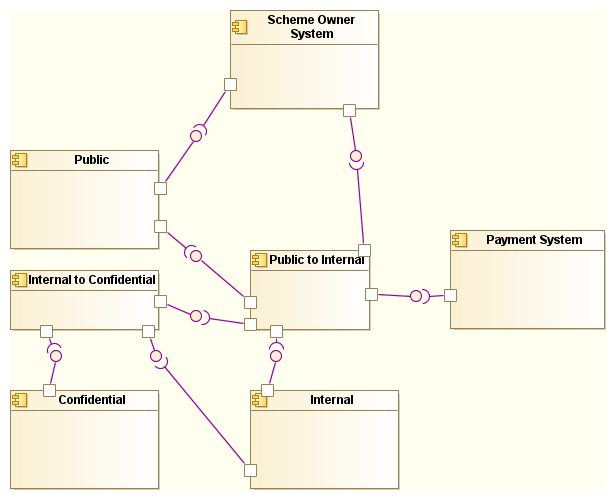
\includegraphics[scale=0.7]{uml/dataarch.png}
    \caption{Aufteilung der Komponenten in Datenbereiche}
\end{figure}

Eine weitere wichtige Regel ist, dass keine Gateways unterschiedlicher Vertrautheitsebenen übersprungen werden dürfen. Zeigt ein Aktivitätsdiagramm zB. einen Zugriff von Ebene 1 auf Ebene 3 muss dieser Zugriff sowohl durch den Gateway der Ebene 2, als auch durch den Gateway der Ebene 3 geleitet werden. Dies verhindert, dass besonders schützenswerte Systeme direkt an Systeme mit einer weitaus niedrigeren Vertrautheitsebene angeschlossen werden und so dessen Gateway zum Single Point of Failure wird. Dies gilt in beide Richtungen.

Da bei der Erstellung des Systems nun alle Schnittstellen und Systeme bekannt sind, können diese Regeln fest im Gateway verankert werden. Weil diese Gateways unabhängig voneinander agieren, können sie durch das Hinzufügen eines Load Balancers beliebig vervielfacht werden, was sowohl die Ausfallsicherheit als auch die Skalierbarkeit erhöht. Das ist wichtig, weil sie als einzige Verbindung zwischen den Systemen zu einer Art Flaschenhals werden.

\section{Einbinden der AkteurInnen}
Nachdem die Datenminimalarchitektur steht, können nun die AkteurInnen des Systems in die Aufgliederung des Systems mit einbezogen werden. Hierfür müssen nun die Objektflüsse und die AkteurInnen des Systems für jeden Usecase betrachtet werden, welche aus den vorher bereits erstellten Aktivitäts- und Kontextdiagramm ersichtlich sind.

Zuerst wird das erste Untersystem, in diesem Falle das Public System, betrachtet. Alle Objektflüsse durch das System und die AkteurInnen, welche mit ihren Swimlanes angrenzen, sind in die Aktivitäten des Systems involviert. Jede Involvierung eines/einer Akteurs/Akteurin in ein System erfordert einen Zugang zu diesem System.

Jeder dieser Akteure muss mit den minimal möglichen Rechten für dieses System ausgestattet werden, um seine Aufgaben zu erfüllen. Dies vermeidet nicht nur Fehler sondern reduziert auch den Schaden, welcher ein potentieller Angriff dieses Akteurs/dieser Akteurin anrichten kann \cite[1. A]{leastpriv}.

Da ein System komplex ist \cite[S. 7]{softarch}, und diese Sicherheitsattribute nach Änderungen am System immer wieder überprüft werden müssen, stellt jeder zusätzliche Zugriff eines/einer Akteurs/Akteurin nicht nur ein Sicherheitsrisiko dar, sondern erhöht auch den Test- und damit den Wartungsaufwand. Idealerweise wird daher jedem/jeder AkteurIn ein eigenes, für sich abgekapseltes System zur Verfügung gestellt, was jedoch meist aufgrund Kosten der zusätzlichen Systeme keine Option dar stellt.

Um zu ermitteln, welche Systeme eine eigene Komponente benötigen, wird nun entweder anhand einer Tabelle oder zusammen mit dem/der KundIn pro Usecase und deren Komponenten ermittelt, ob der Schaden eines unerlaubten Zugriffs der Daten den eines Systems überschreitet. Die Schadens- und Systemkosten müssen zuerst von dem/der KundIn und dem/der ArchitektIn geschätzt werden.

Im Falle des Beispielprojektes wurde auf Basis des folgenden stark vereinfachten Aktivitätsdiagramms in Abbildung \ref{fig:actorarch} ermittelt, dass die möglichen Schadenskosten im Falle, dass der Anwärter (Applicant) Zugriff auf die Prüfungsantworten (Answer) bekommt, die eines eigenen Systems überschreiten. Das gleiche Problem trifft auch auf den Scheme Owner zu: die Schadenskosten im Falle einer Manipulation oder eines lesenden Zugriffes des Anwärters (Applicant) auf die Fragen überschreitet auch hier die Kosten eines eigenen Systems. Deswegen werden zwei zusätzliche Systeme erstellt und aus dem Public System ausgegliedert.

Für den Fall, dass bei der Aufspaltung zu viele Systeme entstanden sind, werden nun in einem weiteren Schritt diverse Kombinationen von Teilsystemen betrachtet und versucht zusammen zu legen, solange deren Schadenskosten nicht die Systemkosten überschreiten. Gibt es mehrere mögliche Kombinationen, entscheidet das in den Anforderungen aufgenommene Related Usecases Feld und danach die Überschneidung der Datentypen über die genaue Aufteilung. Ändert sich ein Usecase, so sind meist auch andere Usecases von dieser Änderung betroffen. Je weniger Komponenten nach einer Änderung betrachtet werden müssen, desto niedriger sind die Wartungskosten.

Beim Beispielprojekt zeigt sich, dass es keine erlaubte Kombination gibt, da die Schadenskosten jeweils weit über den Kosten eines eigenen Systemes liegen. Es bleibt somit bei den ermittelten zwei Zusatzsystemen.

\begin{figure}[H]
    \centering
    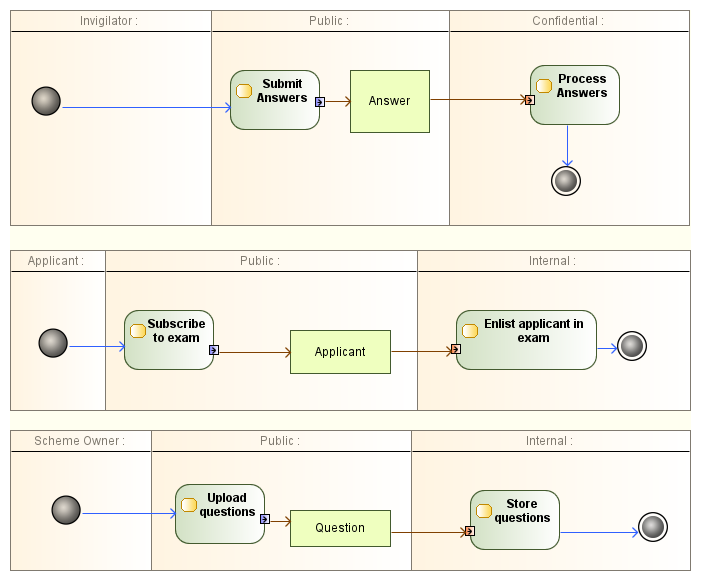
\includegraphics[scale=0.6]{uml/actorarch.png}
    \caption{Vereinfachte Gegenüberstellung von Aktivitätsdiagramme für das Public System}
    \label{fig:actorarch}
\end{figure}

Diese Analyse wird für alle verbleibenden Systeme durchgeführt, bis alle Systeme aufgespalten sind.

Im Falle des Beispielprojektes führt dies schlussendlich zu folgender Systemaufspaltung:

\begin{figure}[H]
    \centering
    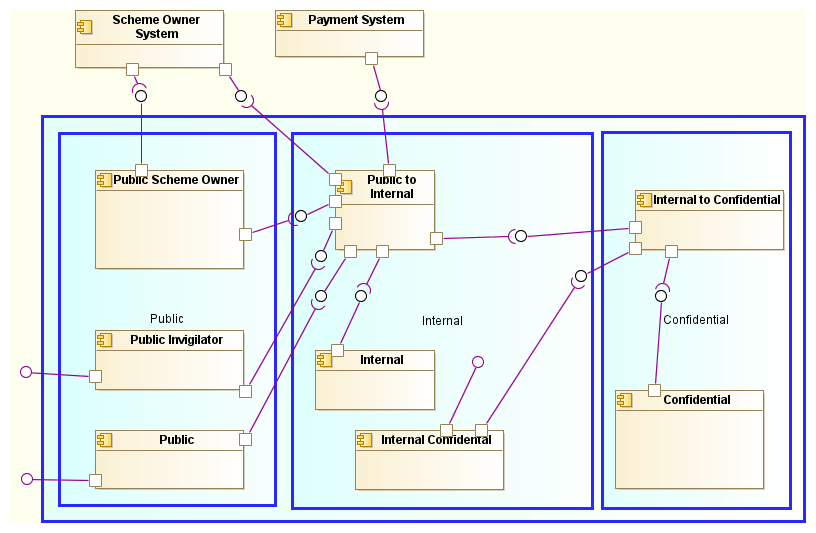
\includegraphics[scale=0.6]{uml/vision4.png}
    \caption{Architektur nach der Aufspaltung }
\end{figure}

\section{Analyse der nicht funktionalen Attribute}
Ist die erste Version der Architektur erstellt, kann nun mit der grundsätzlichen Überprüfung der im Anforderungsprozess ermittelten Parameter begonnen werden, welche bereits wichtige Informationen und Rückschlüsse auf den jetzigen Status der Architektur geben. Basierend auf den Usecases, den ermittelten Komponenten der Architektur und den Aktivitätsdiagrammen wird eine Tabelle erstellt, welche Auskünft darüber gibt, welche Komponenten für jeden Usecase benötigt werden. Diese Tabelle dient als Basis für weitere Analysen.

Um herauszufinden, welche Komponenten für einen Usecase benötigt werden, können die Swimlanes der Aktivitätsdiagramme herangezogen werden. Da für AkteurInnen keine Komponente gelistet werden, werden deren Swimlanes ignoriert. Ein Beispiel hierfür ist das Aktivitätsdiagramm des Handle Complaint Usecases in Abbildung \ref{fig:handlecomplaintreview}.

\begin{figure}[H]
    \centering
    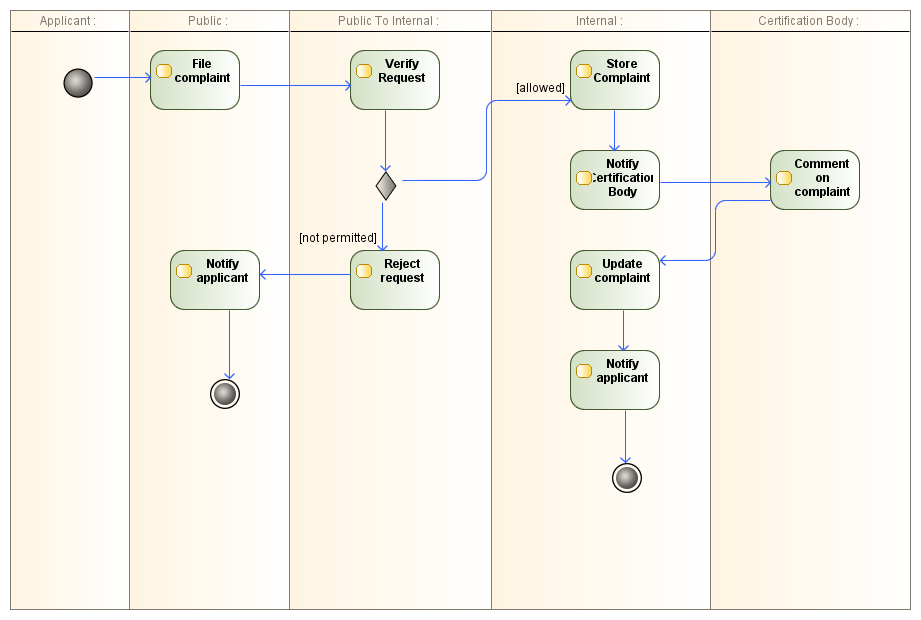
\includegraphics[scale=0.5]{uml/handlecomplaintsactivityreview.png}
    \caption{Vereinfachtes Aktivitätsdiagramm des Handle Complaints Usecases mit der id complaints}
    \label{fig:handlecomplaintreview}
\end{figure}

Werden die beiden AkteurInnen entfernt, bleiben für diesen Usecase folgende Komponenten übrig:

\begin{itemize}
  \item Public
  \item Public To Internal
  \item Internal
\end{itemize}

Diese werden nun in eine Tabelle überführt, wobei für jede verwendete Komponente eines Usecases mit einem x markiert wird:

\hfill \break

\begin{tabular}{ | r | c | }
    \hline
    Komponenten & complaints \\
    \hline
    Public & x \\
    \hline
    Public Invigilator & \\
    \hline
    Public Scheme Owner & \\
    \hline
    Public To Internal & x \\
    \hline
    Internal & x \\
    \hline
    Internal Confidential & \\
    \hline
    Internal To Confidential & \\
    \hline
    Confidential & \\
    \hline
    Scheme Owner System & \\
    \hline
    Payment System & \\
    \hline
\end{tabular}

\hfill \break

Dies wird für alle Usecases durchgeführt und führt im Falle des Beispielprojektes zu folgender Matrix:

\begin{figure}[H]
    \centering
    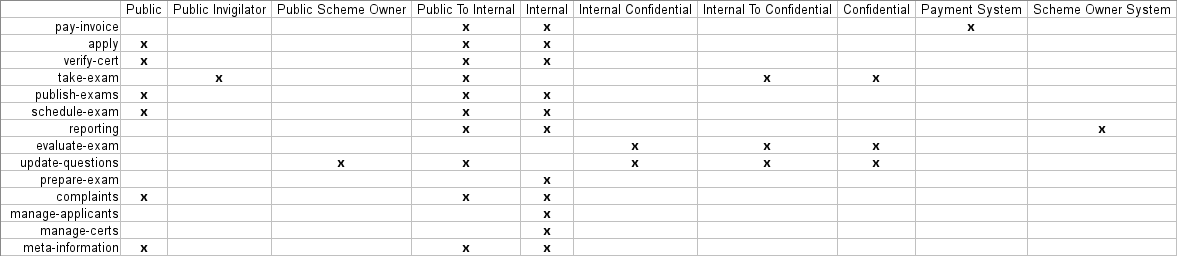
\includegraphics[scale=0.4]{img/matrix.png}
    \caption{Matrix der Komponenten und Usecases des Beispielprojektes}
    \label{fig:matrix}
\end{figure}




\subsection{Reliability}
Anhand der in ermittelten Usecase und Komponenten Matrix kann nun sowohl eine Überprüfung der der Ausfallskosten als auch eine Single Point of Failure Analyse durchgeführt werden.

\subsubsection{Single Point of Failure Analyse}

Ein Single Point of Failure beschreibt eine Komponente, die so kritisch für das System ist, dass ihr Ausfall den kompletten Ausfall des Systems nach sich zieht \cite[S. 3]{single}. Ein Single Point of Failure der Architektur kann daran erkannt werden, dass eine Komponente in allen Usecases vorkommt. Im Bezug auf die soeben ermittelte Matrix wird dies durch eine durchgehende Reihe von mit x markierten Zellen in der Komponentenspalte ersichtlich.

Enthält eine Architektur einen Single Point of Failure, muss diese Komponente entweder redundant ausgelegt sein, oder es muss eine Aufspaltung anhand einer Fehlerkostenanalyse durchgeführt werden.

Im Falle der Matrix in Abbildung \ref{fig:matrix} ist keine durchgehende Reihe an markierten Zellen erkennbar und somit existiert kein Single of Failure. Es lässt sich einzig und allein ablesen, dass die Public To Internal und Internal Komponente eine Abweichung vom Single Point of Failure um vier respektive drei besitzen. Dies lässt erahnen, dass bei der Implementation und Wartung dieser Systeme besondere Sorgfalt von Nöten ist.

\subsubsection{Ausfallkosten Analyse}
Zusätzlich zu einer Single Point of Failure Analyse gibt eine Ausfallkosten Analyse auf Basis des in den Anforderungen ermittelten Monatsumsatzes Auskunft darüber, welche Komponenten jeweils wieviel Umsatz generieren. Für diese Überlegung können auch die Wachstumsszenarien einbezogen werden, falls sich der Umsatz durch eine Steigerung der Benutzer steigert oder senkt.

Die nachfolgenden Berechnungen verteilen den Schaden aus Gründen der Einfachheit gleichmäßig auf alle Zeiteinheiten. Es kann sein, dass eine Organisation so strukturiert ist, dass ein eintägiger Ausfall keine Umsatzeinbußen nach sich zieht. In diesem Falle ist die Beispielrechung ungenau. Um diese Möglichkeit einzubeziehen, müssen detailiertere Umsatzkosten im Anforderungsprozess ermittelt werden was jedoch aus Gründen des Umfangs und der Einfachheit vermieden wird. Das Beispiel soll lediglich als ein anschauliches Beispiel zur Ermitllung des Umsatzrückganges dienen.

Um den monatlichen Umsatz der Komponenten zu ermitteln, wird das x in den markierten Feldern mit dem Monatsumsatz des Usecases ersetzt. Leere Felder werden mit 0 aufgefüllt. Schlussendlich werden alle Werte einer Komponente addiert, um den Gesamtumsatz zu ermitteln.

Als Beispiel dient hier die Internal Komponente:

\hfill \break

\begin{tabular}{ | r | c | }
    \hline
    Usecases & Internal \\
    \hline
    pay-invoice & 3000 \euro \\
    \hline
    apply & 1500 \euro \\
    \hline
    verify-cert & 1500 \euro \\
    \hline
    take-exam & 0 \euro \\
    \hline
    publish-exams & 1500 \euro \\
    \hline
    schedule-exam & 1500 \euro \\
    \hline
    reporting & 1500 \euro \\
    \hline
    evaluate-exam & 0 \euro \\
    \hline
    update-questions & 0 \euro \\
    \hline
    prepare-exam & 80000 \euro \\
    \hline
    complaints & 1500 \euro \\
    \hline
    manage-applicants & 1500 \euro \\
    \hline
    manage-certs & 1500 \euro \\
    \hline
    meta-information & 1500 \euro \\
    \hline
    Total Sum & 96500 \euro \\
    \hline
\end{tabular}

\hfill \break

Fällt diese Komponente für einen kompletten Monat aus, verursacht sie einen Umsatzrückgang von 95500 \euro.

\subsection{Usability}
Da die Artefakte des Planungsprozesses keine Oberflächen beschreiben ist eine Auswertung der des nicht funktionalen Parameters Usability nicht möglich. Die Überprüfung der Usability kann somit übersprungen werden.

\subsection{Efficiency}
Es ist schwierig, die Effizienz und Performance der Architektur in diesem Stadium zu messen, da noch keine Implementation vorhanden ist und somit weder die Performance noch der Speicherverbrauch des Systems getestet werden können. In diesem Stadium lassen sich lediglich Werte schätzen. Eine Möglichkeit um zB. die Antwortzeiten zu schätzen, ist es, die Anzahl der Swimlanewechsel eines Usecases zu addieren und das Ergebnis mit einer konstanten Zeit, welche auf Erfahrungswerten basiert, zu multiplizieren. Dieser Wert kann dann mit den im Anforderungsprozess ermittelten Antwortzeiten verglichen werden, um zu überprüfen, ob das System diese Anforderungen erfüllt.

Ausgegangen wird hier von den bestehenden Aktivitätsdiagrammen. Je nachdem, für welchen Abschnitt die in den Anforderungen ermittelten Werte gelten, kann nicht der komplette Ablauf des Aktivitätsdiagrammes für die Berechnung der Zeit verwendet werden.

Überschreitet der berechnete Wert den in den Anforderungen ermittelten Wert, muss dessen Kategorie hinzugezogen werden. Ist der Wert nur eine Empfehlung, so wird der Usecase in der Implementationsphase mit einem besonderen Augenmerk auf Geschwindigkeit umgesetzt. Ist der Wert jedoch verbindlich, so muss mit dem/der KundIn Rücksprache gehalten werden \cite[S. 70]{effektiv}: Entweder ist die Anforderung unter diesen Parametern nicht umsetzbar, oder es muss ein Kompromiss zu lasten von anderen Anforderungen eingegangen werden.

Ein Beispiel für die Berechnung der Antwortzeiten wird aus dem Aktivitätsdiagramm des Beispielprojektes für die Anmeldung eines Kandidaten erläutert (Abbildung \ref{fig:applycomplicated}):

\begin{figure}[H]
    \centering
    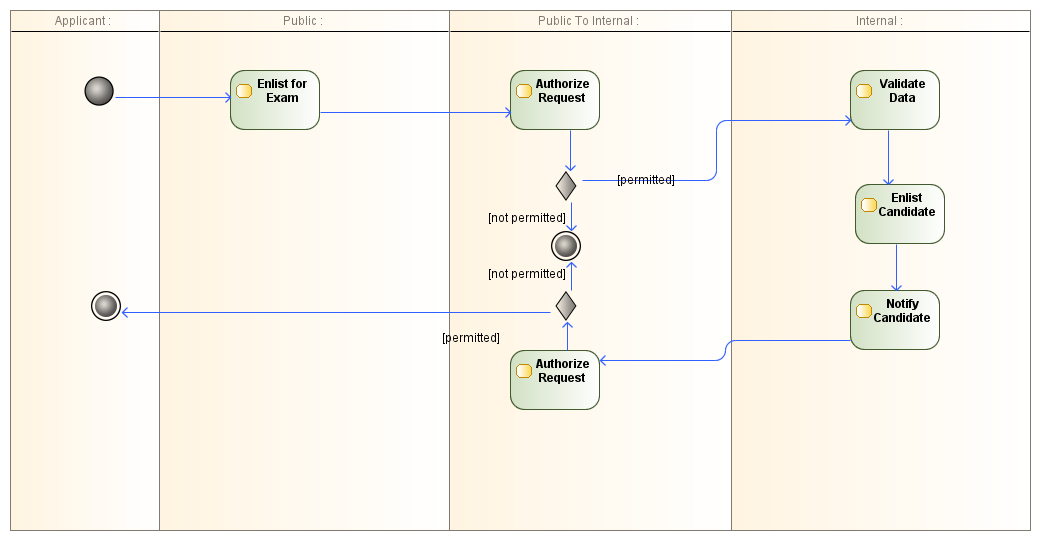
\includegraphics[scale=0.4]{uml/applycomplicated.png}
    \caption{Der Kandidat meldet sich für eine Prüfung an}
    \label{fig:applycomplicated}
\end{figure}

Hier werden, ausgegangen vom Startpunkt sechs Swimlanewechsel gezählt. Diese werden nun mit der Konstante 100 Milisekunden multipliziert, was eine geschätzte Durchlaufzeit von 600 Milisekunden ergibt. Dies liegt unter den erforderlichen 1000 Milisekunden der aufgenommenen nicht funktionalen Anforderung der Antwortzeit.

\subsection{Maintainability}
TBD
Related Usecase Analyse

Wenn man Usecase ändert, alle Komponenten betroffen
Wenn man Komponente ändert, alle anderen Komponenten des Usecases betroffen
-> Usecases mit teurem Ausfallszenario dabei -> eigene Komponente?

Wachstums und Änderungsszenarien mit einbeziehen

\subsection{Portability}
Die Portabilität der Platform kann im Moment noch nicht überprüft werden, da noch keine Festlegung des Projektes auf eine Plattform und/oder Technologie existiert. Dies kann erst zu Beginn der Implementationsphase entschieden werden und wird unter anderem von den in der Anforderungsphase ermittelten Rahmenbedingungen beinflusst.


\section{Modellieren der Komponenten Interfaces (Klassen Diagramm)}
TBD
Aufzeigen dass zb das interne System user anlegen können muss mit methoden im klassendiagramm
